%%
% Plantilla de Memoria
% Modificación de una plantilla de Latex de Nicolas Diaz para adaptarla 
% al castellano y a las necesidades de escribir informática y matemáticas.
%
% Editada por: Mario Román
%
% License:
% CC BY-NC-SA 3.0 (http://creativecommons.org/licenses/by-nc-sa/3.0/)
%%

%%%%%%%%%%%%%%%%%%%%%
% Thin Sectioned Essay
% LaTeX Template
% Version 1.0 (3/8/13)
%
% This template has been downloaded from:
% http://www.LaTeXTemplates.com
%
% Original Author:
% Nicolas Diaz (nsdiaz@uc.cl) with extensive modifications by:
% Vel (vel@latextemplates.com)
%
% License:
% CC BY-NC-SA 3.0 (http://creativecommons.org/licenses/by-nc-sa/3.0/)
%
%%%%%%%%%%%%%%%%%%%%%

%----------------------------------------------------------------------------------------
%	PAQUETES Y CONFIGURACIÓN DEL DOCUMENTO
%----------------------------------------------------------------------------------------

%% Configuración del papel.
% microtype: Tipografía.
% mathpazo: Usa la fuente Palatino.
\documentclass[a4paper, 11pt]{article}
\usepackage[protrusion=true,expansion=true]{microtype}
\usepackage{mathpazo}

% Indentación de párrafos para Palatino
\setlength{\parindent}{0pt}
  \parskip=8pt
\linespread{1.05} % Change line spacing here, Palatino benefits from a slight increase by default


%% Castellano.
% noquoting: Permite uso de comillas no españolas.
% lcroman: Permite la enumeración con numerales romanos en minúscula.
% fontenc: Usa la fuente completa para que pueda copiarse correctamente del pdf.
\usepackage[spanish,es-noquoting,es-lcroman]{babel}
\usepackage[utf8]{inputenc}
\usepackage[T1]{fontenc}
\selectlanguage{spanish}


%% Gráficos
\usepackage{graphics,graphicx, float, url} % Required for including pictures
\usepackage{wrapfig} % Allows in-line images
\usepackage[usenames,dvipsnames]{color} % Coloring code
\usepackage{caption}
\usepackage{subcaption}

% Para algoritmos
\usepackage{algorithm}
\usepackage{algorithmic}
\usepackage{amsthm}
%\floatname{algorithm}{Algoritmo}
\renewcommand{\listalgorithmname}{Lista de algoritmos}
\renewcommand{\algorithmicrequire}{\textbf{Entrada:}}
\renewcommand{\algorithmicensure}{\textbf{Salida:}}
\renewcommand{\algorithmicend}{\textbf{Fin}}
\renewcommand{\algorithmicif}{\textbf{Si}}
\renewcommand{\algorithmicthen}{\textbf{Entonces}}
\renewcommand{\algorithmicelse}{\textbf{En otro caso}}
\renewcommand{\algorithmicelsif}{\algorithmicelse,\ \algorithmicif}
\renewcommand{\algorithmicendif}{\algorithmicend\ \algorithmicif}
\renewcommand{\algorithmicfor}{\textbf{Para }}
\renewcommand{\algorithmicforall}{\textbf{Para cada}}
\renewcommand{\algorithmicdo}{\textbf{}}
\renewcommand{\algorithmicendfor}{\algorithmicend\ \algorithmicfor}
\renewcommand{\algorithmicwhile}{\textbf{Mientras}}
\renewcommand{\algorithmicendwhile}{\algorithmicend\ \algorithmicwhile}
\renewcommand{\algorithmicloop}{\textbf{Repetir}}
\renewcommand{\algorithmicendloop}{\algorithmicend\ \algorithmicloop}
\renewcommand{\algorithmicrepeat}{\textbf{Repetir}}
\renewcommand{\algorithmicuntil}{\textbf{Hasta que}}
\renewcommand{\algorithmicprint}{\textbf{Imprimir}} 
\renewcommand{\algorithmicreturn}{\textbf{Devolver}} 
\renewcommand{\algorithmictrue}{\textbf{Verdadero }} 
\renewcommand{\algorithmicfalse}{\textbf{Falso }} 
\renewcommand{\algorithmicand}{\textbf{Y}}
\renewcommand{\algorithmicor}{\textbf{O}}
\renewcommand{\algorithmicnot}{\textbf{No}}

%% Matemáticas
\usepackage{amsmath}


%% Bibliografía
\makeatletter
\renewcommand\@biblabel[1]{\textbf{#1.}} % Change the square brackets for each bibliography item from '[1]' to '1.'
\renewcommand{\@listI}{\itemsep=0pt} % Reduce the space between items in the itemize and enumerate environments and the bibliography



%----------------------------------------------------------------------------------------
%	TÍTULO
%----------------------------------------------------------------------------------------
% Configuraciones para el título.
% El título no debe editarse aquí.
\renewcommand{\maketitle}{
  \begin{flushright} % Right align
  
  {\LARGE\@title} % Increase the font size of the title
  
  \vspace{50pt} % Some vertical space between the title and author name
  
  {\large\@author} % Author name
  \\\@date % Date
  \vspace{40pt} % Some vertical space between the author block and abstract
  \end{flushright}
}

% Título
\title{\textbf{Prácticas ROS: Robótica}\\ % Title
Entrega 3: Navegación global} % Subtitle

\author{\textsc{Óscar Bermúdez Garrido,\\Iván Calle Gil,\\ Luis Castro Martín,\\ Eva Mª González García} % Author
\\{\textit{Universidad de Granada}}} % Institution

\date{\today} % Date



%----------------------------------------------------------------------------------------
%	DOCUMENTO
%----------------------------------------------------------------------------------------

\begin{document}

\maketitle % Print the title section

% Resumen (Descomentar para usarlo)
\renewcommand{\abstractname}{Resumen} % Uncomment to change the name of the abstract to something else
\begin{abstract}

\end{abstract}

% Palabras clave
%\hspace*{3,6mm}\textit{Keywords:} lorem , ipsum , dolor , sit amet , lectus % Keywords
%\vspace{30pt} % Some vertical space between the abstract and first section

% Índice
{\parskip=2pt
  \tableofcontents
}
\pagebreak

%% Inicio del documento

\section{Implementación del algoritmo A*}
	

\section{Mejora del algoritmo A*}
	Para mejorar el \textbf{algoritmo A*}, optamos por introducir la variación de peso mediante la
	ponderación por la máxima distancia disponible en el mapa.
	
	Esto es, el peso de nuestra variación sería:
	$$\omega = \frac{\texttt{distancia al objetivo}}{\texttt{distancia máxima del mapa}} \cdot 3 + 1$$

\section{Pruebas en distintos mapas}
	\subsection{laberinto}
		\subsubsection{Algoritmo A*}
			En esta ejecución, se obtuvo un tiempo de 12.0125 s con el siguiente recorrido:
			\begin{figure}[H]
				\centering
				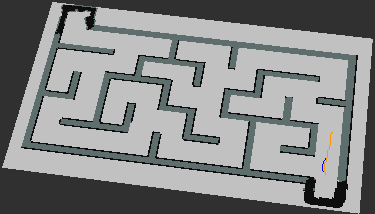
\includegraphics[width=6cm]{Pruebas/A*/laberinto/laberinto(1)-1}
				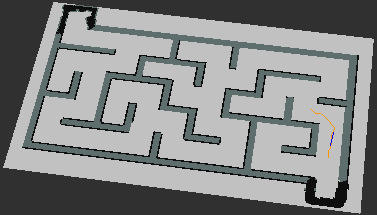
\includegraphics[width=6cm]{Pruebas/A*/laberinto/laberinto(1)-2}
				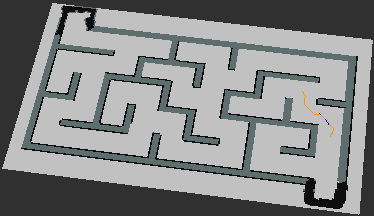
\includegraphics[width=6cm]{Pruebas/A*/laberinto/laberinto(1)-3}
				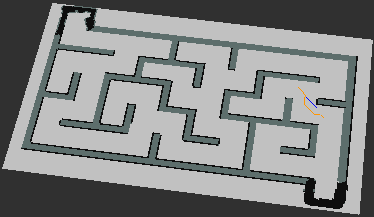
\includegraphics[width=6cm]{Pruebas/A*/laberinto/laberinto(1)-4}
				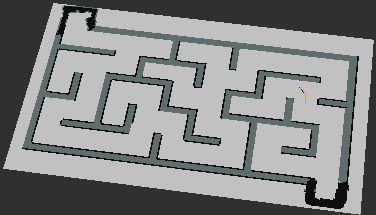
\includegraphics[width=6cm]{Pruebas/A*/laberinto/laberinto(1)-5}
				\caption{Recorrido del robot.}
				\label{A-lab}
			\end{figure}
			
		\subsubsection{Mejora del algoritmo A*}
			En esta ejecución, se aprecia una pequeña mejora, dando como resultados un tiempo de 10.9578 s
			y el recorrido: 
			
			\begin{figure}[H]
				\centering
				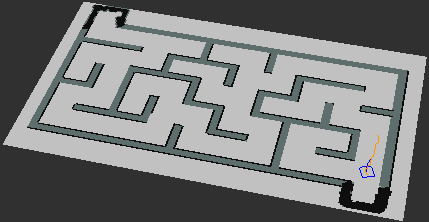
\includegraphics[width=6cm]{Pruebas/Mejora-A*/laberinto/laberinto(2)-1}
				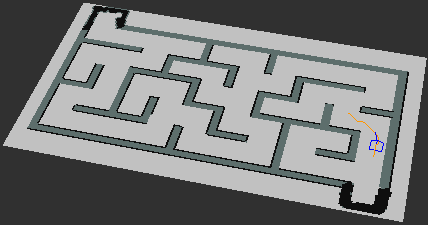
\includegraphics[width=6cm]{Pruebas/Mejora-A*/laberinto/laberinto(2)-2}
				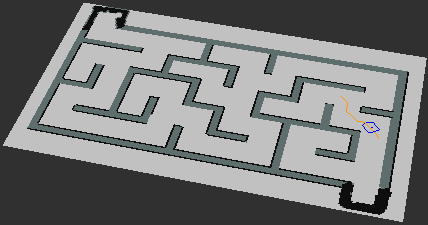
\includegraphics[width=6cm]{Pruebas/Mejora-A*/laberinto/laberinto(2)-3}
				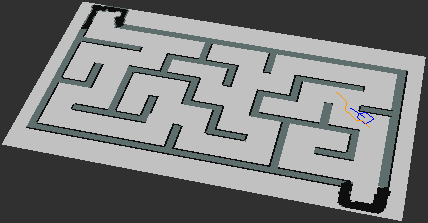
\includegraphics[width=6cm]{Pruebas/Mejora-A*/laberinto/laberinto(2)-4}
				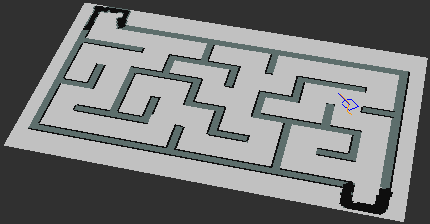
\includegraphics[width=6cm]{Pruebas/Mejora-A*/laberinto/laberinto(2)-5}
				\caption{Recorrido del robot.}
				\label{MA-lab}
			\end{figure}
	\subsection{simplerooms}
		\subsubsection{Algoritmo A*}
			En esta ejecución, se obtuvo un tiempo de 32.4385 s siguiendo el camino:
			\begin{figure}[H]
				\centering
				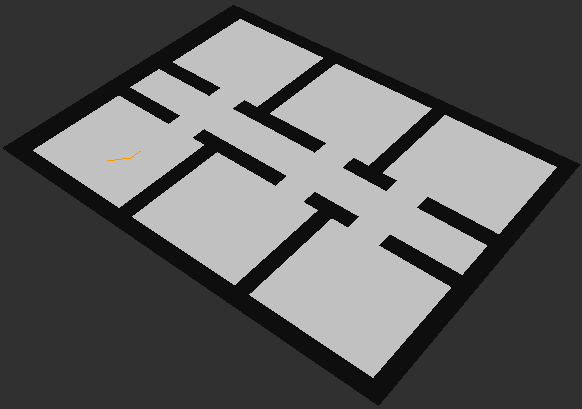
\includegraphics[width=6cm]{Pruebas/A*/simplerooms/simplerooms(1)-1}
				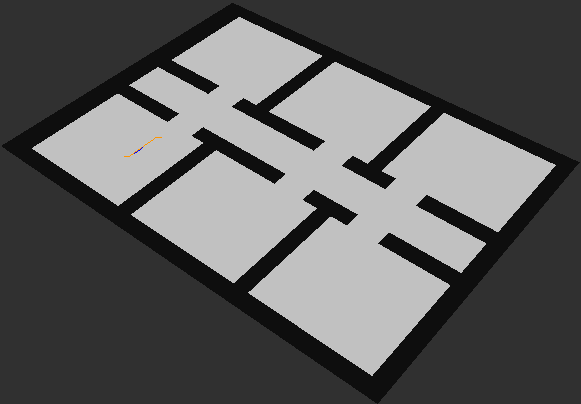
\includegraphics[width=6cm]{Pruebas/A*/simplerooms/simplerooms(1)-2}
				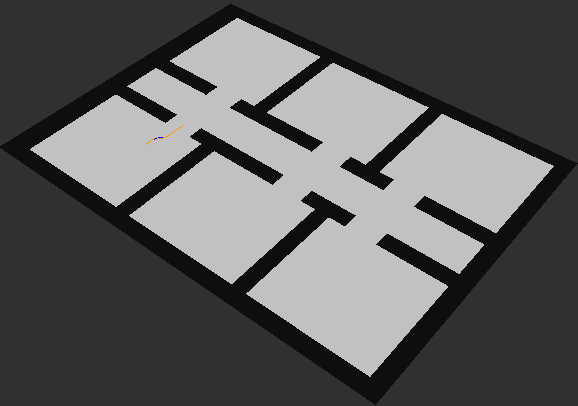
\includegraphics[width=6cm]{Pruebas/A*/simplerooms/simplerooms(1)-3}
				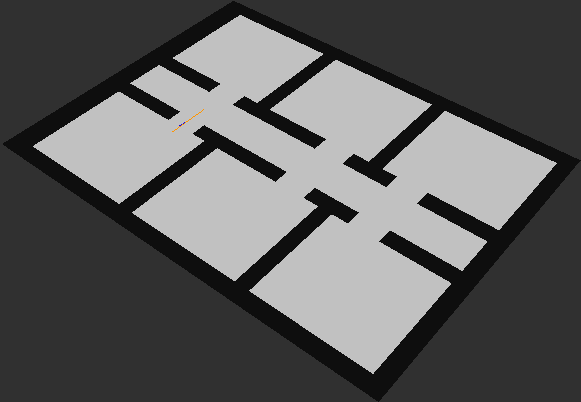
\includegraphics[width=6cm]{Pruebas/A*/simplerooms/simplerooms(1)-4}
				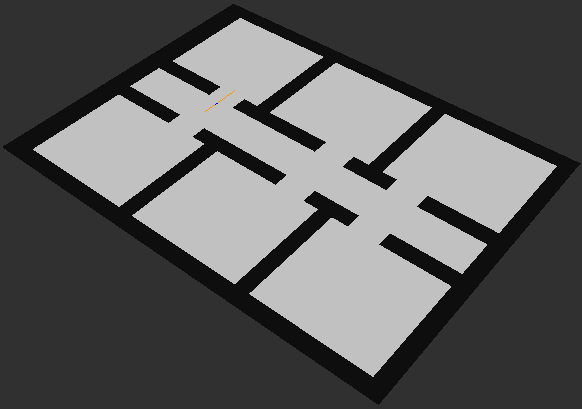
\includegraphics[width=6cm]{Pruebas/A*/simplerooms/simplerooms(1)-5}
				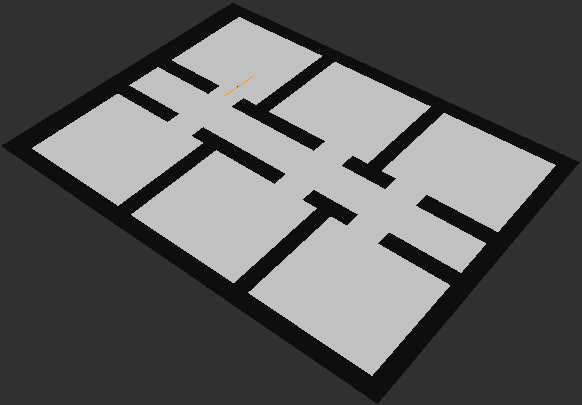
\includegraphics[width=6cm]{Pruebas/A*/simplerooms/simplerooms(1)-6}
				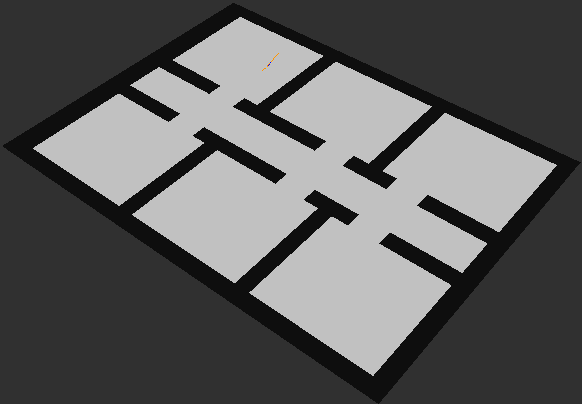
\includegraphics[width=6cm]{Pruebas/A*/simplerooms/simplerooms(1)-7}
				\caption{Recorrido del robot.}
				\label{A-sim}
			\end{figure}
			
		\subsubsection{Mejora del algoritmo A*}
			En esta ejecución, se aprecia un ligero empeoramiento, con un tiempo de 32.7008 s y ruta: 

			\begin{figure}[H]
				\centering
				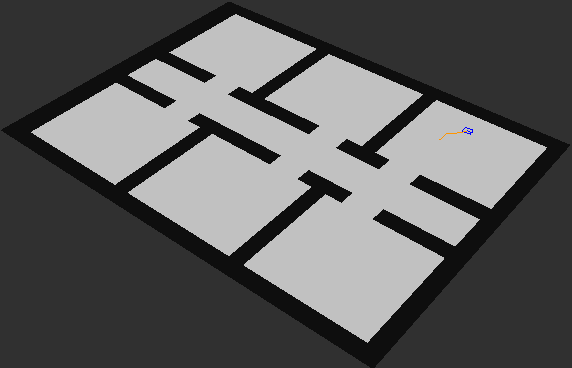
\includegraphics[width=6cm]{Pruebas/Mejora-A*/simplerooms/simplerooms(2)-1}
				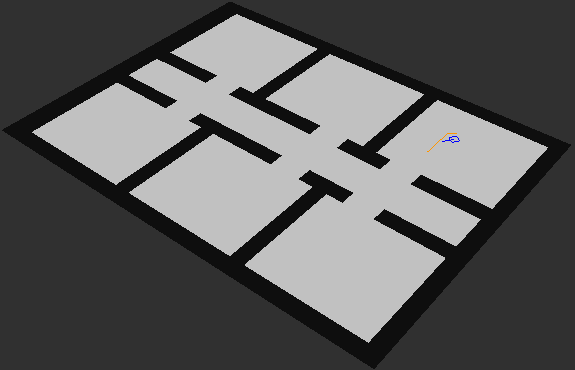
\includegraphics[width=6cm]{Pruebas/Mejora-A*/simplerooms/simplerooms(2)-2}
				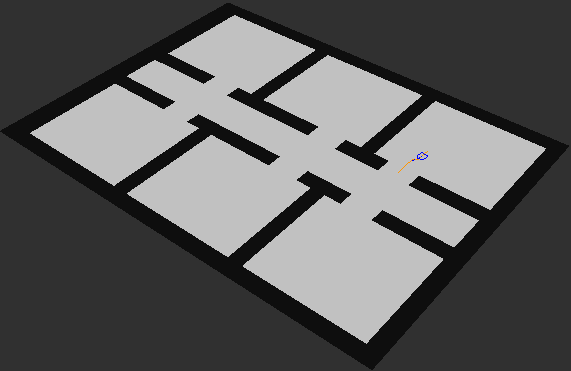
\includegraphics[width=6cm]{Pruebas/Mejora-A*/simplerooms/simplerooms(2)-3}
				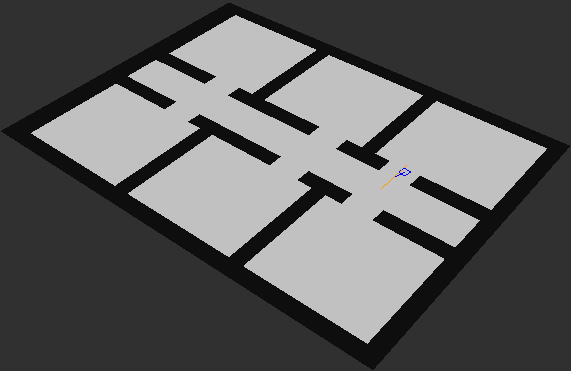
\includegraphics[width=6cm]{Pruebas/Mejora-A*/simplerooms/simplerooms(2)-4}
				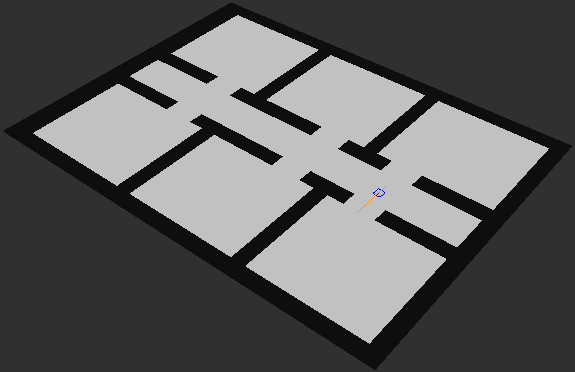
\includegraphics[width=6cm]{Pruebas/Mejora-A*/simplerooms/simplerooms(2)-5}
				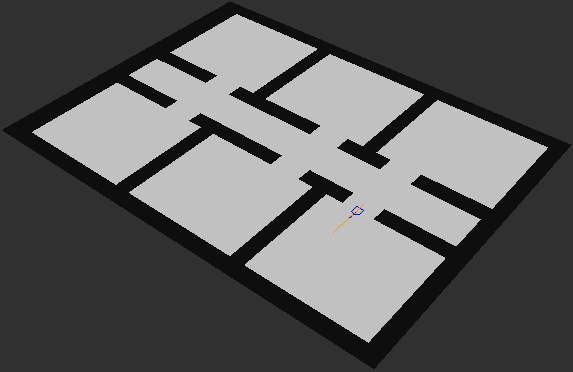
\includegraphics[width=6cm]{Pruebas/Mejora-A*/simplerooms/simplerooms(2)-6}
				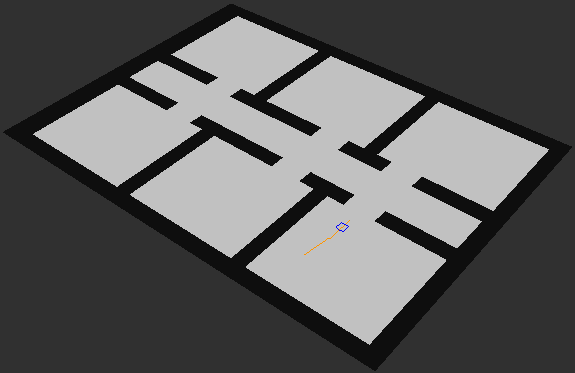
\includegraphics[width=6cm]{Pruebas/Mejora-A*/simplerooms/simplerooms(2)-7}
				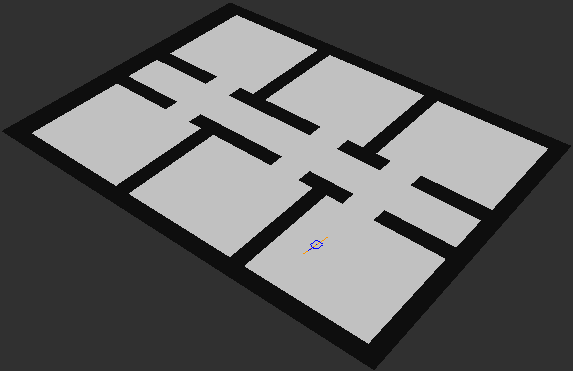
\includegraphics[width=6cm]{Pruebas/Mejora-A*/simplerooms/simplerooms(2)-8}
				\caption{Recorrido del robot.}
				\label{MA-sim}
			\end{figure}
			
	\subsection{willow}
		\subsubsection{Algoritmo A*}
			En esta ejecución, el tiempo fue 25.7184 s con el recorrido:
			\begin{figure}[H]
				\centering
				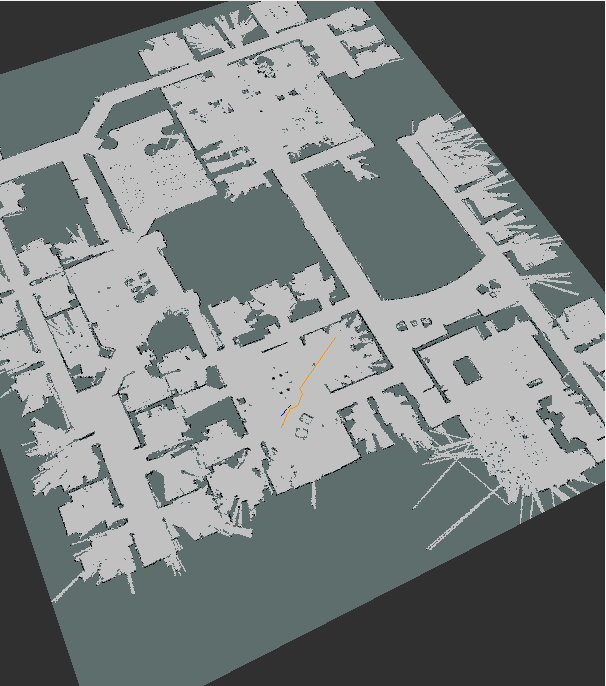
\includegraphics[width=6cm]{Pruebas/A*/willow/willow(1)-1}
				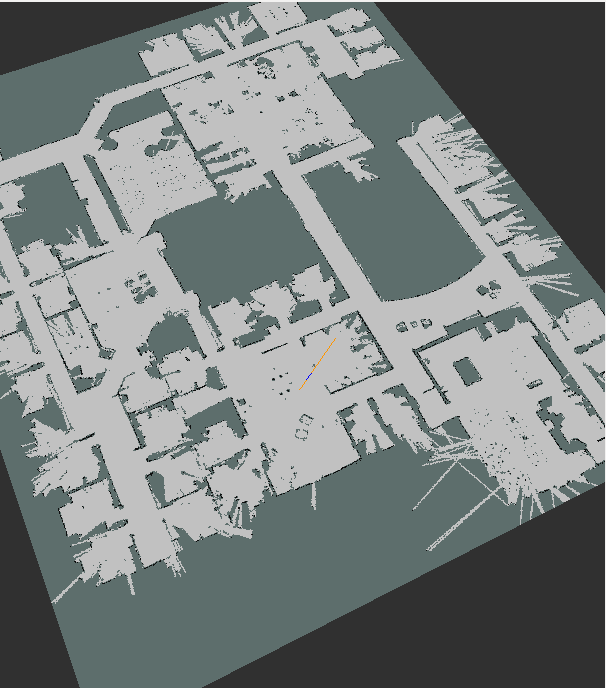
\includegraphics[width=6cm]{Pruebas/A*/willow/willow(1)-2}
				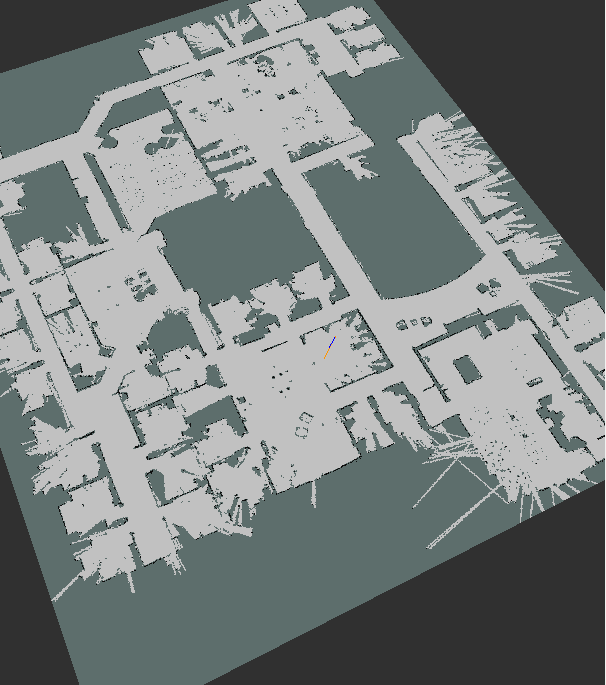
\includegraphics[width=6cm]{Pruebas/A*/willow/willow(1)-3}
				\caption{Recorrido del robot.}
				\label{A-wil}
			\end{figure}
			
		\subsubsection{Mejora del algoritmo A*}
			En esta ejecución, se aprecia una gran mejora con la incorporación de los pesos, dando como
			resultados un tiempo de 13.5573 s y el recorrido: 
			
			\begin{figure}[H]
				\centering
				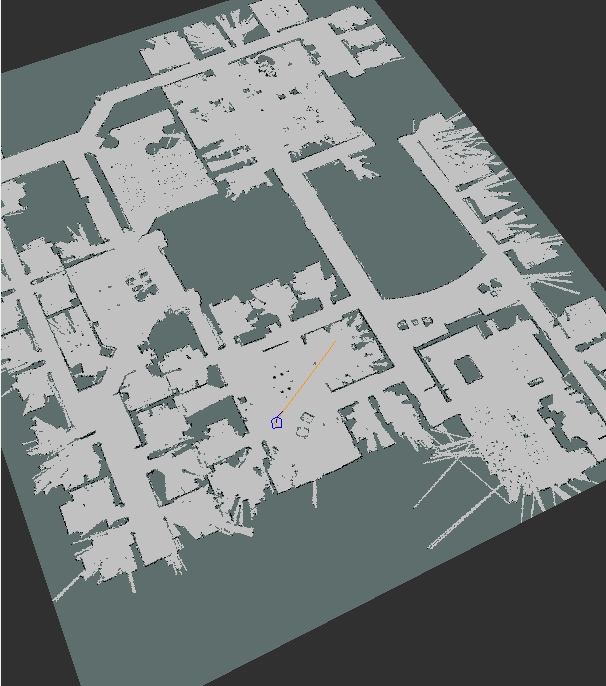
\includegraphics[width=6cm]{Pruebas/Mejora-A*/willow/willow(2)-1}
				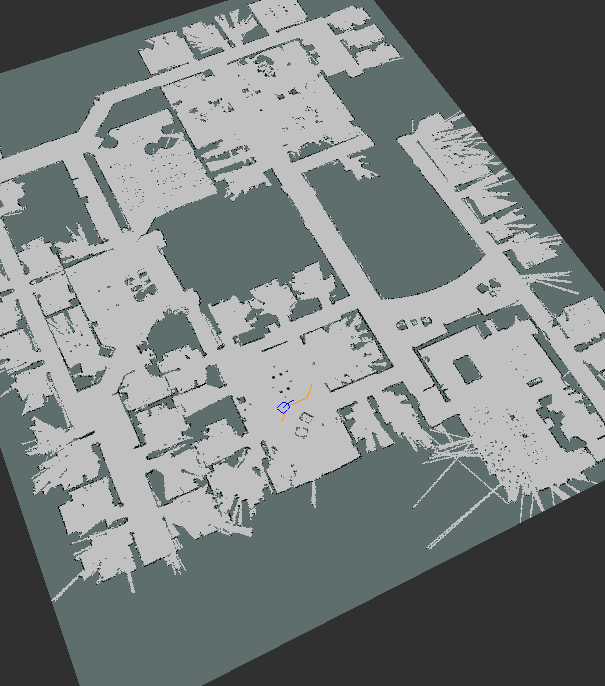
\includegraphics[width=6cm]{Pruebas/Mejora-A*/willow/willow(2)-2}
				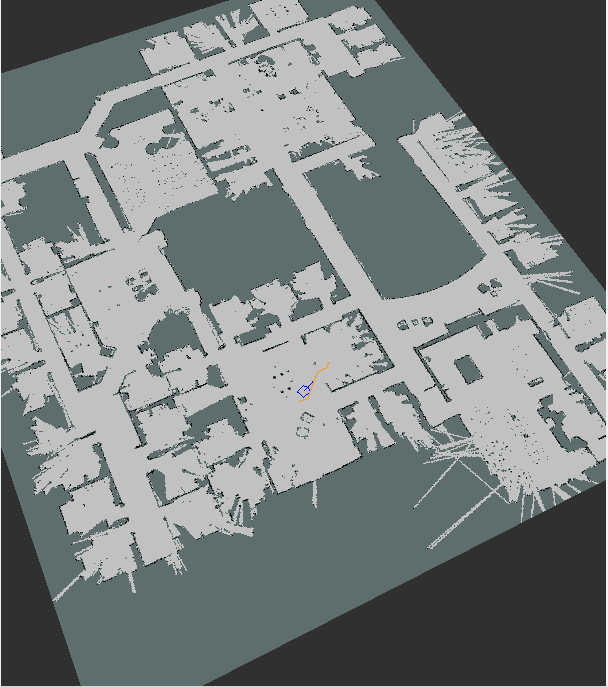
\includegraphics[width=6cm]{Pruebas/Mejora-A*/willow/willow(2)-3}
				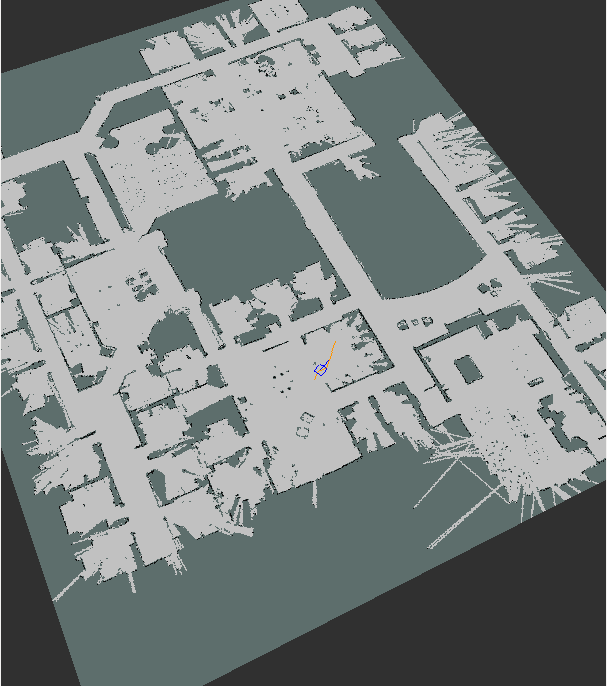
\includegraphics[width=6cm]{Pruebas/Mejora-A*/willow/willow(2)-4}
				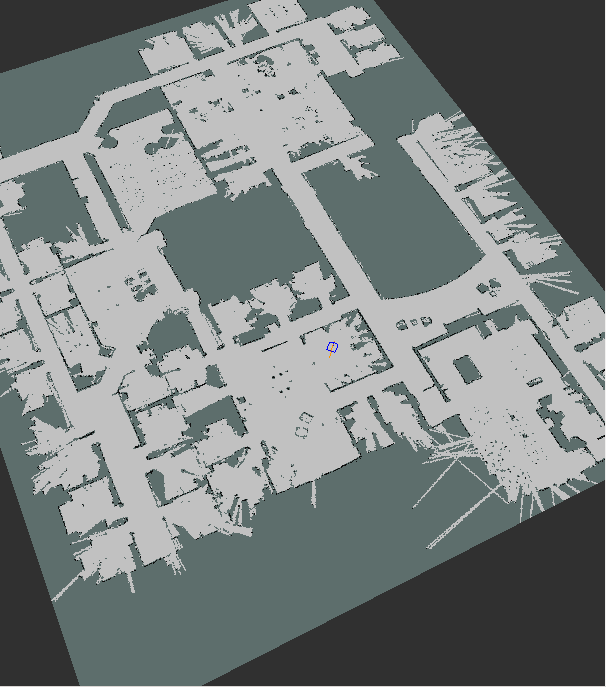
\includegraphics[width=6cm]{Pruebas/Mejora-A*/willow/willow(2)-5}
				\caption{Recorrido del robot.}
				\label{MA-wil}
			\end{figure}
	
\end{document}
